% locobench_phase2.tex
% LoCoBench Phase 2: the data-generation harness.
% Companion to locobench_phase1.tex (the framework); this document specifies the
% harness that executes it and the run protocol.
% Compile: pdflatex locobench_phase2.tex (run twice).
%
% Phase 1 = the FRAMEWORK (facets, error taxonomy, prompts, schema, metrics).
% Phase 2 = THIS: the generation harness, the run protocol, and the cost model.
%
% Two Phase-1 spec defects are corrected here (Section 1.3); both were found by
% attempting to encode Phase 1 as executable assertions.

\documentclass[11pt]{article}

\usepackage[margin=1in]{geometry}
\usepackage{amsmath}
\usepackage{amssymb}
\usepackage{enumitem}
\usepackage[table]{xcolor}
\usepackage{booktabs}
\usepackage{array}
\usepackage[numbers,square]{natbib}
\usepackage{tikz}
\usetikzlibrary{arrows.meta,positioning,calc,backgrounds,fit,shapes.geometric}
\usepackage[colorlinks=true,urlcolor=blue!60!black,linkcolor=blue!60!black,
            citecolor=blue!60!black]{hyperref}

\definecolor{cGen}  {RGB}{210,228,248}   % generation stage
\definecolor{cVal}  {RGB}{215,236,219}   % validation gate
\definecolor{cStore}{RGB}{250,219,180}   % persistence
\definecolor{cFix}  {RGB}{248,205,205}   % a correction to Phase 1

\newcommand{\cEnt}{\textsc{entailment}}
\newcommand{\cCon}{\textsc{contradiction}}
\newcommand{\cEqv}{\textsc{equivalence}}
\newcommand{\cExc}{\textsc{exclusive}}
\newcommand{\cCoN}{\textsc{co\_necessity}}
\newcommand{\cNone}{\textsc{none}}
\newcommand{\readout}[1]{\texttt{#1}}
\newcommand{\pymod}[1]{\texttt{#1}}

% This document is dense with unhyphenatable identifiers; prefer loose spacing to
% lines in the margin.
\sloppy
\emergencystretch=3em

\title{LoCoBench Phase 2: The Data-Generation Harness\\
       \large Pipeline, validation committee, resume protocol, cost model
       --- and two corrections to the Phase-1 contracts}
\author{FactReasoner --- Ideation}
\date{\today}

\begin{document}
\maketitle

\begin{abstract}\noindent
Phase 1 fixed \emph{what} LoCoBench is: five facets, 36 subject topics over four domains, four
family types, six perturbation operators, a five-prompt generation pipeline with four validators,
a gold schema and the metrics. It deferred the run. This document specifies \emph{how} the corpus
is produced: a resumable harness, \pymod{src/fact\_reasoner/locobench/}, driven by one command, and
the protocol for using it. The design target is a harness that is cheap to iterate on --- it runs
end to end with no LLM and no Merlin --- and safe to interrupt, because a 600-item corpus at
$\approx$65 model calls per family is a run measured in days, and the recovery move after any
failure must be to type the same command again. Three things make it usable: \textbf{resume is the
default}, \textbf{every acceptance threshold lives in one auditable table}, and \textbf{every gate
failure is recorded with a reason rather than silently retried}. Two Phase-1 defects surfaced while
encoding its contracts as executable assertions, and both would have produced checks that can
never pass: the C1 ordering contract demands a strict increase in \readout{log\_partition} at a rung
where the reference ladder itself shows no change, and the schema's \texttt{topic} field holds a
free-text framing that cannot be checked against the hard 36-topic coverage constraint. Both are
corrected here, in Section~\ref{sec:defects}.
\end{abstract}

\tableofcontents

% =====================================================================================
\section{What Phase 2 delivers}
\label{sec:scope}

\subsection{Scope}

Phase 1 closes with the canonical statement of this phase's job:

\begin{quote}
``Phase 2 is the generation run: topic selection, the live prompt pipeline, the validation
committee, and the harness that turns \texttt{expected} blocks into assertions.''
\end{quote}

Those four parts map onto this document as Sections~\ref{sec:pipeline} (topic selection and the
prompt pipeline), \ref{sec:committee} (the committee), \ref{sec:store} (the assertions, as the
\texttt{expected} blocks the harness emits) and \ref{sec:cost} (what the run costs before
committing to it, which Phase-1 R6 asks for explicitly).

The deliverable is two things: this document, and the package
\pymod{src/fact\_reasoner/locobench/}. The corpus it produces is
\textbf{120 families $\times$ 5 rungs = 600 items}, $\approx$4{,}800 gold relations, with all 36
topics represented and a floor of three families each.

\subsection{What Phase 2 does \emph{not} change}

The facets, the taxonomy, the prompt texts, the schema and the metrics are Phase-1 artefacts and
are treated here as fixed. Where this document specifies a prompt, it is the Phase-1 text
verbatim; the harness holds those strings as module constants and a test asserts they still match
Phase 1's instruction count and placeholder set, so the two cannot drift
(Section~\ref{sec:milestones}).

Two Phase-1 items are also deliberately left alone. \readout{reified} stays out of scope, though
the harness \emph{records} it per item as a diagnostic, which Phase 1 §6.1 explicitly permits.
And Restatement's $0.90$ strength prior stays untested as a contract; what the harness does is
report the distribution of mined strength on gold Restatement edges, which is the empirical
question R4 actually poses.

\subsection{Two corrections to the Phase-1 contracts}
\label{sec:defects}

Encoding Phase 1's ordering contracts and coverage constraints as executable assertions surfaced
two defects. Neither is a modelling error; both are places where the specification, taken
literally, cannot be satisfied. They are stated first because the harness's data structures depend
on the resolutions.

\paragraph{Defect 1 --- the C1 contract is unsatisfiable at rung 1$\to$2 for
\readout{log\_partition}.}
Phase 1 §5.3 assigns \readout{mean\_marginal} and \readout{log\_partition} to contract C1: a strict
increase across \emph{all four} adjacent rung pairs. But the reference ladder in Phase 1
(\texttt{tab:rungs}) reports, from an exact $2^{16}$-world enumeration of the AeroParts model:

\begin{table}[h]\centering\small
\renewcommand{\arraystretch}{1.1}
\begin{tabular}{@{}clcc@{}}
\toprule
\textbf{Rung} & \textbf{Name} & \textbf{\readout{mean\_marginal}} & \textbf{$\log Z$}\\
\midrule
1 & \texttt{base}                 & $0.607$ & $-9.64$\\
\rowcolor{cFix}
2 & \texttt{concession\_resolved} & $0.612$ & $-9.64$ \quad\emph{(unchanged)}\\
\bottomrule
\end{tabular}
\caption{The offending pair, from Phase 1's own reference ladder. \readout{mean\_marginal} rises;
$\log Z$ does not move at all, so a contract demanding a \emph{strict} increase in
\readout{log\_partition} here cannot be met by any correct implementation.}
\label{tab:defect1}
\end{table}

The reason is structural, and it is the same mechanism behind Phase-1 Finding 1. The concession
edit changes an edge's \emph{weight} ($p{=}0.80 \to 0.55$), not the edge \emph{set}. The
normalized log-partition readout measures the base $\log Z$ against a ceiling built by removing
contradictions and a floor built by saturating them --- and both bounds are constructed from the
\emph{same edge skeleton} as the base. A weight-only change can therefore leave the normalized
quantity fixed, exactly as it leaves \readout{consistency} free to invert.

\noindent\textbf{Resolution.} The 1$\to$2 step becomes a \emph{predicted invariance} for
\readout{log\_partition}, asserted as $|\Delta| \leq 2\sigma$ rather than $\Delta > 2\sigma$. C1
still governs its other three adjacent pairs. Concretely, the harness emits ordering expectations
\textbf{per readout per adjacent pair}, never as one chain-wide flag --- which is the data-structure
consequence, and the reason this defect had to be settled before writing \pymod{store.py}. Phase 1
§5.3 carries an erratum note pointing here.

\paragraph{Defect 2 --- \texttt{meta.topic} cannot be checked against the coverage constraint.}
Phase 1 requires that \textbf{every one of the 36 topics} contribute families, with a floor of
three. But the schema's example item carries
\begin{center}
\texttt{"topic": "aviation component failure investigation"}
\end{center}
which is a P1 \emph{framing} string, not one of the 36 canonical labels (the canonical label for
that item is \emph{Civil Engineering}). As written, the hard coverage constraint is unverifiable:
nothing in an item says which of the 36 buckets it belongs to.

\noindent\textbf{Resolution.} The item schema gains \texttt{meta.canonical\_topic}, drawn from the
36, alongside the free-text \texttt{meta.framing} that P1 produced. \pymod{topics.py} is the single
source of truth for the grid, and the coverage check is a query over
\texttt{canonical\_topic}. Both fields are kept: the framing is what makes the question specific,
the canonical label is what makes coverage checkable.

\subsection{Smaller inconsistencies, settled}

Five further ambiguities do not change the harness's structure but would otherwise be resolved
differently by different implementers. They are settled here, in the document, so the code has one
reading to follow.

\begin{table}[h]\centering\small
\renewcommand{\arraystretch}{1.15}
\begin{tabular}{@{}lp{5.4cm}p{6.2cm}@{}}
\toprule
& \textbf{The ambiguity} & \textbf{Settled as}\\
\midrule
1 & \textsc{v3}'s attachment: the pipeline figure draws its gate from \textsc{p5}, the prompt
    index lists it under \textsc{p4} & \textsc{v3} runs on \emph{every} response text, base and
    perturbed. It is the cheapest validator and the one whose failure mode (annotation leakage)
    can be introduced by a perturbation\\
2 & \textsc{v5}'s voter set: §7.2 says the committee runs \textsc{v1}/\textsc{v2}/\textsc{v4};
    the figure's box fits \textsc{v4}/\textsc{v2}/\textsc{v3} & §7.2 is normative. \textsc{v1},
    \textsc{v2}, \textsc{v4} are voted; \textsc{v3} is a single-model audit\\
3 & \textsc{p2}'s composition: instruction 3 mandates 24 claims $+$ 2 holdings, the worked
    exemplar shows 17 & The instruction wins; the exemplar is abbreviated for the page. The parser
    validates against instruction 3\\
4 & \textsc{o5}'s inverse is named \texttt{add\_resolution} in the manifest but only
    \texttt{remove\_resolution} in §4.2 & Both registered. \texttt{remove\_resolution} builds the
    unresolved rung, \texttt{add\_resolution} the resolved one\\
5 & Topic floor: the \texttt{tab:topics} caption says ``at least one family'', the allocation
    paragraph says three & Three. The caption understates the constraint the allocation rule
    actually imposes\\
\bottomrule
\end{tabular}
\caption{Ambiguities in Phase 1 settled by this document. None requires a Phase-1 edit beyond the
Defect-1 erratum; they are recorded so the harness has a single reading.}
\label{tab:ambiguities}
\end{table}

% =====================================================================================
\section{The harness at a glance}
\label{sec:harness}

\subsection{One command}

The normal way to use the harness is one command, and the recovery move after any failure is the
same command again:

\begin{center}\small
\begin{tabular}{@{}ll@{}}
\toprule
\textbf{Command} & \textbf{What it does}\\
\midrule
\texttt{locobench-generate -{}-config locobench.json} & the run; re-run to resume\\
\texttt{locobench-generate -{}-dry-run -{}-limit 2}   & full pipeline, no LLM, no Merlin\\
\texttt{locobench-generate ... -{}-only-topic Law}    & one topic, for inspection\\
\texttt{locobench-generate ... -{}-stage plan}        & stop after \textsc{p3}\\
\texttt{locobench-generate ... -{}-report}            & coverage and cost, generate nothing\\
\bottomrule
\end{tabular}
\end{center}

Three properties make that safe, and they are the harness's actual design requirements rather
than nice-to-haves:

\begin{enumerate}[leftmargin=*,nosep,label=(\arabic*)]
  \item \textbf{Resume is the default.} Every run reads the existing output directory first and
        prints what it found (\texttt{431/600 items, 12 gate failures, resuming}). Completed
        families are skipped; only gate failures and unstarted families are worked. There is no
        \texttt{-{}-resume} flag because there is no non-resuming mode.
  \item \textbf{Dry-run covers the whole pipeline.} \texttt{-{}-dry-run} substitutes a
        deterministic offline generator for the LLM and the brute-force oracle for Merlin, so the
        parsers, gates, ladders, schema assertions and storage all execute. A developer can
        exercise every code path in seconds without credentials.
  \item \textbf{Failures are recorded, not retried silently.} A family failing a gate is written
        to \texttt{rejected/} with the validator, the threshold and the observed value. Nothing is
        discarded, and the rejection rate per gate is itself a reportable finding about the
        prompts.
\end{enumerate}

\subsection{The stage machine}

\begin{figure}[h]
\centering
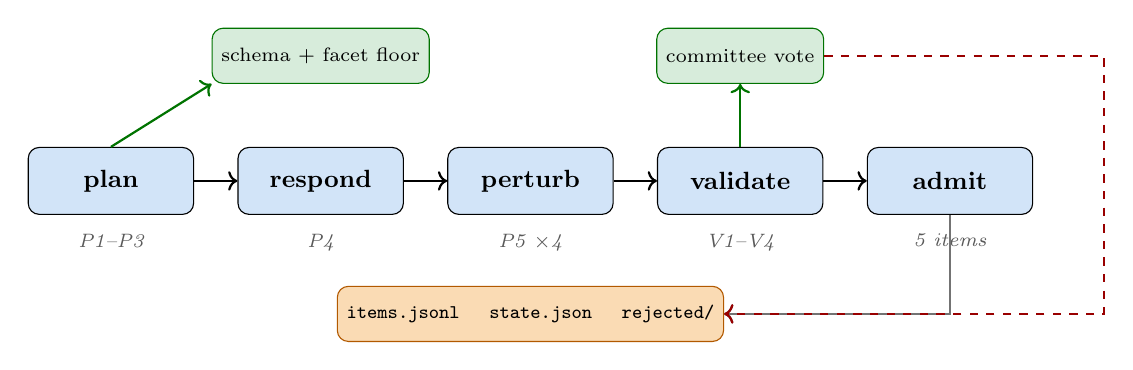
\begin{tikzpicture}[
  node distance=5.5mm,
  stage/.style={draw,rounded corners,minimum height=8.5mm,minimum width=21mm,
                font=\small\bfseries,fill=cGen},
  gate/.style={draw,rounded corners,minimum height=7mm,minimum width=17mm,
               font=\scriptsize,fill=cVal,draw=green!45!black},
  store/.style={draw,rounded corners,minimum height=7mm,font=\scriptsize,fill=cStore,
                draw=orange!70!black},
  art/.style={font=\scriptsize\itshape,text=black!65},
  flow/.style={->,thick},
  chk/.style={->,green!45!black,thick},
  rej/.style={->,red!60!black,thick,dashed},
]
\node[stage] (plan)   {plan};
\node[stage,right=of plan]    (resp) {respond};
\node[stage,right=of resp]    (pert) {perturb};
\node[stage,right=of pert]    (val)  {validate};
\node[stage,right=of val]     (adm)  {admit};
\draw[flow] (plan) -- (resp);
\draw[flow] (resp) -- (pert);
\draw[flow] (pert) -- (val);
\draw[flow] (val)  -- (adm);

\node[art,below=1.2mm of plan] {P1--P3};
\node[art,below=1.2mm of resp] {P4};
\node[art,below=1.2mm of pert] {P5 $\times$4};
\node[art,below=1.2mm of val]  {V1--V4};
\node[art,below=1.2mm of adm]  {5 items};

\node[gate,above=8mm of resp] (g1) {schema $+$ facet floor};
\node[gate,above=8mm of val]  (g2) {committee vote};
\draw[chk] (plan.north) -- (g1.south west);
\draw[chk] (val.north)  -- (g2.south);

\node[store,below=9mm of pert] (st) {\texttt{items.jsonl} \quad \texttt{state.json} \quad
                                     \texttt{rejected/}};
\draw[flow,black!55] (adm.south) |- (st.east);
\draw[rej] (g2.east) -| ($(adm.east)+(9mm,0)$) |- (st.east);
\end{tikzpicture}
\caption{The five stages, the two gate points, and the store. Each stage is resumable at family
granularity: \texttt{state.json} records the last stage a family completed, so an interrupted run
restarts it there rather than from \texttt{plan}. The dashed edge is the rejection path --- a
family failing the committee vote is stored with its reason, not dropped.}
\label{fig:stages}
\end{figure}

\subsection{The modules}

\begin{table}[h]\centering\small
\renewcommand{\arraystretch}{1.15}
\begin{tabular}{@{}lp{10.4cm}@{}}
\toprule
\textbf{Module} & \textbf{Responsibility}\\
\midrule
\pymod{config.py}   & \texttt{GenConfig} and \texttt{load\_config(path)}. JSON by default (stdlib);
  YAML accepted only when \texttt{yaml} imports, since it is \emph{not} a declared dependency of
  this project. \texttt{to\_dict()} travels with the output for provenance\\
\pymod{topics.py}   & the 36 topics $\times$ 4 domains as the single source of truth, and
  \texttt{allocate(n)} implementing the three-per-topic floor and the surplus rule\\
\pymod{prompts.py}  & \textsc{p1}--\textsc{p5}, \textsc{v1}--\textsc{v4} as module constants with
  \texttt{\{\{placeholder\}\}} slots, verbatim from Phase 1 Appendix A\\
\pymod{parse.py}    & one parser per prompt output. Every parser returns
  \texttt{(value, error)} and never raises, so a malformed generation is a gate failure rather
  than a crash\\
\pymod{perturb.py}  & \textsc{o1}--\textsc{o6}, the eleven parameterized calls, and the four family
  ladders as declarative rung recipes\\
\pymod{validate.py} & the committee, the aggregation rules, the agreement statistics, and the single
  \texttt{THRESHOLDS} table\\
\pymod{schema.py}   & item and manifest validators, including the
  \texttt{COMPILE[sense].level1 == coupling} assertion and the real
  \texttt{candidate\_pairs.select} call that fills window admission\\
\pymod{store.py}    & append-only \texttt{items.jsonl}, the family manifest, \texttt{state.json},
  and \texttt{rejected/}\\
\pymod{pipeline.py} & \texttt{generate\_family(topic, cfg)} --- the stage machine of
  Figure~\ref{fig:stages}\\
\pymod{mock.py}     & the deterministic offline generator behind \texttt{-{}-dry-run}\\
\pymod{cli.py}      & \texttt{locobench-generate}\\
\bottomrule
\end{tabular}
\caption{The harness modules. It is a sibling of \pymod{fact\_reasoner/experiments/}, not an
extension of it: that package is a stateless sweep that rewrites every cell, whereas generation is
stateful, gated and resumable. The scoring sweep stays where it is.}
\label{tab:modules}
\end{table}

\paragraph{What is reused rather than rebuilt.} \texttt{utils.run\_throttled} for bounded-concurrency
fan-out --- it already captures per-item exceptions instead of propagating them, which is exactly
the failure isolation a long run needs; \texttt{backends.build\_backend} for every model;
\texttt{cli.\_add\_backend\_args} and \texttt{\_backend\_context} so model selection matches the
other two commands; \texttt{lcs.taxonomy.COMPILE} as the authority for sense$\to$coupling;
\texttt{lcs.candidate\_pairs.select} for window admission; and
\texttt{experiments.mock.dry\_run\_patches} for the offline scoring path.

% =====================================================================================
\section{The generation pipeline, stage by stage}
\label{sec:pipeline}

Each stage below states its inputs, the prompt it issues, what the parser must extract, the gate
that admits its output, and --- the part Phase 1 leaves open --- \textbf{what happens on failure}.
The failure column is what makes the harness a harness rather than a script.

\begin{table}[h]\centering\small
\renewcommand{\arraystretch}{1.2}
\begin{tabular}{@{}llp{3.9cm}p{5.5cm}@{}}
\toprule
\textbf{Stage} & \textbf{Prompt} & \textbf{Gate} & \textbf{On failure}\\
\midrule
plan    & \textsc{p1} & question is bracketed, non-empty &
  \textbf{retry} up to 3$\times$, then skip the topic slot and log\\
plan    & \textsc{p2} & 24 claims $+$ 2 holdings; all tags present &
  \textbf{retry} 3$\times$; a missing \texttt{[alt-pair]} or \texttt{[holding]} is fatal to the
  family, since the rare facets depend on them\\
plan    & \textsc{p3} & JSON schema-valid; $\geq$1 each of Alternative, Disjunction, Restatement,
  Concession, Precedence/Succession; every edge within 4 positions or entity-sharing; 55/45
  validity &
  \textbf{regenerate} the plan 3$\times$. Persistent failure rejects the family with the unmet
  clause named\\
respond & \textsc{p4} & $\geq$500 words; then \textsc{v1}, \textsc{v3}, \textsc{v4} &
  \textbf{regenerate} the response, keeping the plan. \textsc{v1} shortfall may instead
  \textbf{drop the unrecovered edges} from gold (never keep them)\\
perturb & \textsc{p5} & exactly one operator applied; length drift $\leq$15\%; JSON diff parses &
  \textbf{retry} the single rung 3$\times$; a rung that will not build rejects the family, since a
  ladder with a hole carries no ranking claim\\
validate & \textsc{v1}--\textsc{v4} & the thresholds of Table~\ref{tab:thresholds} &
  \textbf{reject} to \texttt{rejected/} with validator, threshold and observed value\\
admit   & --- & schema assertion; window admission recomputed on realized text &
  \textbf{reject}; a schema violation is a harness bug and is surfaced loudly\\
\bottomrule
\end{tabular}
\caption{The stages and their failure policies. Three distinct responses to failure --- retry the
call, regenerate the artefact, or reject the family --- and the choice is not arbitrary: retry for
transient parse failures, regenerate when the artefact is wrong but its inputs are fine, reject
when the family cannot carry its ranking claim. Only \textsc{v1} has a fourth option (drop the
offending edges), and only because Phase 1 mandates it: unrecovered edges must never be retained
as gold.}
\label{tab:stages}
\end{table}

\subsection{Topic selection}

\pymod{topics.py} owns the grid. \texttt{allocate(120)} gives every one of the 36 topics three
families ($36 \times 3 = 108$) and distributes the remaining twelve to the topics that best support
the scarce relation facets --- Law, Medicine, Civil Engineering, Political Science and Ethics ---
because those are where exhaustive alternatives and adjudicating holdings occur naturally. The
three-family floor holds without exception; the surplus is the only discretionary part, and it is
recorded in the manifest so a reader can see where the corpus is deliberately denser.

Each family draws one canonical topic and asks \textsc{p1} for a framing within it. Both are
stored (Defect 2): \texttt{canonical\_topic} for the coverage query,
\texttt{framing} for provenance.

\subsection{A worked family}

One \textsc{conflict} family, from topic to five admitted items, with the call count:

\begin{enumerate}[leftmargin=*,nosep,label=\arabic*.]
  \item \textbf{plan.} \textsc{p1} on \emph{Civil Engineering} returns a framing about
        third-party component failure with competing explanations (1 call). \textsc{p2} returns 26
        tagged claims including an \texttt{[alt-pair]} (``no one was harmed'' / ``three passengers
        died'') and two \texttt{[holding]} claims (1 call). \textsc{p3} returns a JSON plan: 16
        atoms, 10 relations covering all five required senses, 5 non-relations (1 call, up to 3 on
        regeneration).
  \item \textbf{respond.} \textsc{p4} realizes the plan as $\geq$500 words of prose (1 call).
  \item \textbf{perturb.} \textsc{p5} calls build rungs 0, 2, 3, 4 from the base
        (Section~\ref{sec:ladders}); rung 1 \emph{is} the base and costs nothing. This is
        \textbf{7 calls} for a \textsc{conflict} ladder rather than 4, because a single rung may
        compose several operator calls --- summing \pymod{perturb.LADDERS} is the only reliable way
        to count them.
  \item \textbf{validate.} \textsc{v1}, \textsc{v2}, \textsc{v4} run on all five items across
        four committee models --- the generator is excluded. \textsc{v1}, \textsc{v3} and
        \textsc{v4} additionally run \emph{inline} on the base response under the generator model,
        as the stage's own gate. This is the bulk of the cost, and Section~\ref{sec:cost} counts it.
  \item \textbf{admit.} Five items written to \texttt{items.jsonl}, one manifest entry with its
        ordering constraints, and the family marked complete in \texttt{state.json}.
\end{enumerate}

\noindent If any rung fails, the family is rejected \emph{whole}. A four-rung ladder cannot carry
the ranking claim that is the family's only purpose, so partial families are not admitted --- this
is why the gate sits at family granularity and not item granularity.

% =====================================================================================
\section{Perturbation and the ladders}
\label{sec:ladders}

\subsection{Operators to calls}

The six operators of Phase 1 §4.2 are the vocabulary a reader needs; the harness dispatches the
eleven parameterized calls the \textsc{p5} prompt accepts. \pymod{perturb.py} holds the
mapping as a table, so adding a call never requires touching the prompt:

\begin{table}[h]\centering\small
\renewcommand{\arraystretch}{1.15}
\begin{tabular}{@{}llp{7.3cm}@{}}
\toprule
\textbf{Op} & \textbf{Meaning} & \textbf{Calls}\\
\midrule
\textsc{o1} & relabel        & \texttt{wrong\_sense(edge, new\_sense)},
  \texttt{direction\_reversal(edge)}, \texttt{exhaustiveness\_flip(edge)}\\
\textsc{o2} & add conflict   & \texttt{inject\_contradiction(atom)},
  \texttt{spurious\_relation(atom\_a, atom\_b)}\\
\textsc{o3} & break chain    & \texttt{break\_chain(edge)}\\
\textsc{o4} & drop relation  & \texttt{drop\_relation(edge)}\\
\textsc{o5} & resolve/unresolve & \texttt{remove\_resolution(edge)},
  \texttt{add\_resolution(edge)}\\
\textsc{o6} & reorder        & \texttt{shuffle\_order(level)}, \texttt{ordering\_only(edge)}\\
\bottomrule
\end{tabular}
\caption{The operator-to-call mapping. \texttt{add\_resolution} is registered explicitly
(ambiguity 4 of Table~\ref{tab:ambiguities}): the manifest names it, Phase 1 §4.2 mentions only
its inverse, and the resolved rung of every \textsc{conflict} ladder needs it.}
\label{tab:opcalls}
\end{table}

\subsection{The four ladders, as recipes}

Each family type is a declarative list of five rung recipes. \pymod{perturb.py} holds them as data,
which is what lets \pymod{store.py} emit the per-pair expectations mechanically.

\begin{table}[h]\centering\small
\renewcommand{\arraystretch}{1.15}
\begin{tabular}{@{}lrp{8.9cm}@{}}
\toprule
\textbf{Family} & \textbf{$n$} & \textbf{Rungs 0$\to$4 (each derived from the base unless noted)}\\
\midrule
\textsc{conflict} & 55 &
  \texttt{spurious\_relation} $|$ \emph{base} $|$ \texttt{add\_resolution} $|$
  \texttt{add\_resolution}$+$\texttt{drop\_relation} $|$ all conflicts dropped\\
\textsc{chain}    & 25 &
  \texttt{break\_chain}$\times$3 $|$ $\times$2 $|$ $\times$1 $|$ \emph{base} $|$ coherent rewrite\\
\textsc{order}    & 25 &
  \texttt{shuffle\_order(full)} $|$ \texttt{(block)} $|$ \texttt{(adjacent)} $|$ \emph{base} $|$
  \texttt{ordering\_only} \emph{(flat rung)}\\
\textsc{control}  & 15 &
  five meaning-preserving edits: \texttt{ordering\_only} and \texttt{direction\_reversal} only.
  The required pattern is a \textbf{flat line}\\
\bottomrule
\end{tabular}
\caption{The four ladders. \textsc{control} is the family whose correct result is \emph{no}
trend; it is what distinguishes a coherence score from a score that tracks edit count, and it is
the one a hurried implementation would omit.}
\label{tab:ladders}
\end{table}

\subsection{The expectations the harness emits}

For every family the harness writes an \texttt{expected} block per item and an
\texttt{ordering\_constraints} list per family. Per Defect 1 these are \textbf{per readout per
adjacent pair}, and for the \textsc{conflict} ladder they come out as:

\begin{table}[h]\centering\small
\renewcommand{\arraystretch}{1.15}
\begin{tabular}{@{}lcccc@{}}
\toprule
\textbf{Adjacent pair} & \textbf{0$\to$1} & \textbf{1$\to$2} & \textbf{2$\to$3} &
\textbf{3$\to$4}\\
\midrule
\readout{mean\_marginal} & increase & increase & increase & increase\\
\rowcolor{cFix}
\readout{log\_partition} & increase & \textbf{invariant} & increase & increase\\
\readout{consistency}    & increase & \textbf{decrease} & unconstrained & increase\\
\bottomrule
\end{tabular}
\caption{The \textsc{conflict} ladder's ordering expectations. The shaded cell is Defect 1's
resolution: an \emph{invariance} assertion where Phase 1 §5.3 demanded an increase. The
\readout{consistency} row is Phase 1's Finding 1 unchanged --- the predicted inversion, asserted
rather than exempted. Only \readout{mean\_marginal} is monotone across the whole chain, which is
why it is the headline readout.}
\label{tab:expectations}
\end{table}

\noindent Three readouts, four pairs, and the three rows differ: that is the content of Phase 1's
per-readout contract design, and it is the reason \texttt{readout\_directions} is a
$3 \times 4$ structure in the schema rather than a single label per rung.

% =====================================================================================
\section{The validation committee}
\label{sec:committee}

\subsection{The panel, and why the generator is excluded}

Five models from at least three distinct families run \textsc{v1}, \textsc{v2} and \textsc{v4}
independently at temperature 0. \textsc{v3} is a single-model audit (ambiguity 1 of
Table~\ref{tab:ambiguities}). Per-edge labels are decided by majority, except the \cExc\ label,
which requires unanimity.

The constraint that shapes the implementation is \textbf{per-item generator exclusion}: the model
that ran \textsc{p3}/\textsc{p4} for an item may not vote on it. This is Phase-1 R3, and it is not
a formality --- a model asked to recover relations from prose it wrote itself recovers its own
lexical fingerprints, which inflates every Target-A number. So the committee is chosen per item,
not per run, and \pymod{validate.py} takes the panel and the generator identity together:

\begin{center}\small
\texttt{committee\_for(item) = [m for m in cfg.committee if m != item.provenance.planned\_by]}
\end{center}

With a five-model panel and one generator excluded, four models vote on any given item. The
harness therefore requires $\geq$4 usable committee models to reach a majority of three, and
refuses to start a run configured with fewer --- a check at config-load time rather than a
surprise at item 400.

\paragraph{The cross-generation control.} The harness stratifies generators across $\geq$3
families and records \texttt{planned\_by} per item, so Target-A metrics can be reported both
pooled and restricted to items whose generator family differs from the miner's. Phase 1 asks for
that gap to be published as a bias estimate; making it computable is a storage requirement, met by
carrying \texttt{planned\_by} in provenance.

\subsection{Every threshold, in one table}

These are the Phase-1 acceptance criteria, gathered here because a run's behaviour is entirely
determined by them and they should be auditable in one place. \pymod{validate.py} holds this as a
single \texttt{THRESHOLDS} dict; there are no thresholds elsewhere in the harness.

\begin{table}[h]\centering\small
\renewcommand{\arraystretch}{1.12}
\begin{tabular}{@{}llp{6.55cm}@{}}
\toprule
\textbf{Key} & \textbf{Value} & \textbf{Meaning, and the action on breach}\\
\midrule
\multicolumn{3}{@{}l}{\emph{Per-item admission}}\\
\texttt{v1\_coupling} & $\geq 0.80$ & fraction of planned relations recovered with the correct
  coupling; breach $\Rightarrow$ drop the unrecovered edges or regenerate\\
\texttt{v1\_sense}    & $\geq 0.70$ & same, for sense\\
\texttt{v1\_rule}     & majority    & of the committee must meet both rates\\
\texttt{v2\_exclusive} & unanimity  & required to assign an \cExc\ gold label; split vote
  $\Rightarrow$ ship the edge \texttt{low\_agreement}\\
\texttt{v3\_scores}   & all $\geq 4$ & fluency, formality, organization on 1--5\\
\texttt{v3\_spans}    & empty       & \texttt{leakage} and \texttt{hedging} must both be empty
  (\texttt{artifacts} is recorded, not gated)\\
\texttt{v4\_coverage} & $=1.00$     & every atom \texttt{asserted}; any
  altered/missing/merged $\Rightarrow$ regenerate\\
\midrule
\multicolumn{3}{@{}l}{\emph{Plan structure (\textsc{p3})}}\\
\texttt{claims} / \texttt{relations} / \texttt{non\_relations} & 14--18 / 8--12 / 4--6 &
  selected atoms, planned edges, distractor pairs\\
\texttt{validity\_split} & $0.55/0.45$ & valid to invalid, per family\\
\texttt{window}       & 4 positions & or a shared named entity; re-verified on realized text\\
\texttt{rare\_facets} & $\geq 1$ each & Alternative, Disjunction, Restatement, Concession, and one
  of Precedence/Succession\\
\midrule
\multicolumn{3}{@{}l}{\emph{Perturbation (\textsc{p5})}}\\
\texttt{length\_drift} & $\leq 15\%$ & except $\pm$1 sentence for
  \texttt{inject\_contradiction} / \texttt{remove\_resolution} / \texttt{break\_chain}\\
\midrule
\multicolumn{3}{@{}l}{\emph{Corpus-level, checked by \texttt{-{}-report}}}\\
\texttt{topic\_floor} & $\geq 3$ families & for each of the 36 canonical topics, no exception\\
\texttt{none\_pool}   & $\geq 1{,}500$ & in-window distractor pairs across the corpus\\
\midrule
\multicolumn{3}{@{}l}{\emph{Agreement (\textsc{v5}), measured on the human subsample}}\\
\texttt{kappa\_coupling} & $\geq 0.70$ & Fleiss' $\kappa$, 6-way\\
\texttt{kappa\_sense}    & $\geq 0.60$ & Fleiss' $\kappa$, 13-way\\
\texttt{kappa\_exhaustive} & $\geq 0.55$ & Cohen's $\kappa$, binary; the expected weak point,
  reported separately\\
\texttt{alpha\_strength} & --- & Krippendorff's $\alpha$, ordinal, on strength bands\\
\midrule
\multicolumn{3}{@{}l}{\emph{Scoring margins (used by the metrics, not by admission)}}\\
\texttt{margin} & $2\sigma$ & $\sigma$ over 5 re-mines of the same rung; below it a constraint is
  \texttt{indeterminate} and leaves the denominator\\
\bottomrule
\end{tabular}
\caption{The \texttt{THRESHOLDS} table. A facet whose agreement falls below its $\kappa$ floor
ships flagged \texttt{low\_agreement}: excluded from headline metrics, but reported --- an
unreliable facet is itself a result about the taxonomy, which is why the harness must not silently
drop it.}
\label{tab:thresholds}
\end{table}

\subsection{The human subsample}

Three annotators on 120 items (20\%), stratified to cover \emph{all} \cExc\ and \cCoN\ gold edges,
\emph{all} resolved Concessions, and \emph{all} ordering-only invariance rungs, plus a random
remainder. The stratification is not a convenience: those are precisely the facets with no prior
gold data and the highest expected model unreliability, so uniform sampling would spend the human
budget on the categories that need it least. \pymod{validate.py} exposes
\texttt{stratified\_sample(items, n=120)} implementing exactly that rule, so the sample is
reproducible from the corpus rather than chosen by hand.

Human-versus-committee agreement is what licenses the committee as a human proxy on the other
80\%, so it is reported whether or not it clears the floors.

% =====================================================================================
% Float barrier: keep this section's tables inside it.
\clearpage

\section{Storage, resume and provenance}
\label{sec:store}

\subsection{On-disk layout}

\begin{center}\small
\begin{tabular}{@{}ll@{}}
\toprule
\textbf{Path} & \textbf{Contents}\\
\midrule
\texttt{items.jsonl}      & one admitted item per line, keyed by \texttt{id}\\
\texttt{families.json}    & the manifest: rungs, operators, ordering constraints, $\sigma$\\
\texttt{state.json}       & per family: last completed stage, gate verdicts, attempt counts\\
\texttt{rejected/}        & one JSON per rejected family: the validator, threshold, observed value\\
\texttt{config.json}      & the resolved \texttt{GenConfig} snapshot, for provenance\\
\bottomrule
\end{tabular}
\end{center}

\texttt{items.jsonl} is append-only and \texttt{state.json} is rewritten atomically after each
family, which is the same discipline \texttt{CoherenceRunner.assess\_file} uses: the output is
always a valid corpus, even if the process dies mid-run.

\subsection{The resume algorithm}

\begin{enumerate}[leftmargin=*,nosep,label=\arabic*.]
  \item Read \texttt{state.json}. Every family with \texttt{stage == "admitted"} is done.
  \item Every family in \texttt{rejected/} is retried \emph{if} its attempt count is below the
        limit, and reported as permanently rejected otherwise.
  \item Every family in an intermediate stage restarts \emph{at that stage}, reusing the artefacts
        already stored --- a family that has a validated plan does not re-plan.
  \item Unstarted allocation slots are generated.
  \item Print the banner, then work only what steps 2--4 identified.
\end{enumerate}

\noindent The consequence worth stating: \textbf{a completed run is a fixed point}. Running the
command again does nothing and costs nothing, which is what makes it safe to put in a loop or a
cron job while a long generation finishes.

\subsection{Provenance carried per item}

Enough to answer, later, why any given gold label is what it is: which model planned the item and
which wrote its response (\texttt{planned\_by}), which models recovered each edge and how they
voted (\texttt{recovered\_by}, \texttt{exhaustiveness\_votes}), whether a human confirmed it, the
per-validator scores, and the \texttt{window\_admission} verdict computed by the real
\texttt{candidate\_pairs.select} call rather than assumed. This is what makes the cross-generation
bias control of Section~\ref{sec:committee} computable after the fact.

% =====================================================================================
\section{Cost model}
\label{sec:cost}

Phase-1 R6 asks that the run be costed before committing to 600 items. The figures below are
\emph{measured from the harness}, not estimated: call counts come from summing
\pymod{perturb.LADDERS} and instrumenting a full \texttt{-{}-dry-run} over one family of each type,
and token volumes come from counting the rendered prompt and the mock response for every prompt
identifier. This matters, because the hand-derived breakdown in an earlier draft of this section was
wrong in two places --- it assumed a flat 4 \textsc{p5} calls per family and counted \textsc{v2} per
item --- and the corrected total is lower, not higher.

\begin{table}[h]\centering\small
\renewcommand{\arraystretch}{1.15}
\begin{tabular}{@{}lrrp{5.4cm}@{}}
\toprule
\textbf{Stage} & \textbf{Per family} & \textbf{Corpus} & \textbf{Note}\\
\midrule
\textsc{p1} question        & 1        & 120   & per family\\
\textsc{p2} claims          & 1        & 120   & \\
\textsc{p3} plan            & 1        & 120   & up to 3 on regeneration\\
\textsc{p4} response        & 1        & 120   & up to 3 on \textsc{v1}/\textsc{v3}/\textsc{v4} failure\\
\textsc{p5} perturbation    & 7 / 4    & 720   & \textbf{7} for \textsc{conflict} and
  \textsc{chain}, \textbf{4} for \textsc{order} and \textsc{control}: a rung may compose several
  operator calls\\
\midrule
\textsc{v1} recovery (inline) & 1      & 120   & base response, generator model\\
\textsc{v3} audit             & 1      & 120   & base response, single-model\\
\textsc{v4} coverage (inline) & 1      & 120   & base response, generator model\\
\midrule
\textsc{v1} recovery (panel)  & 20     & 2{,}400 & 5 items $\times$ 4 non-generator voters\\
\textsc{v4} coverage (panel)  & 20     & 2{,}400 & \\
\textsc{v2} exhaustiveness    & 12     & 1{,}440 & 3 conflict edges $\times$ 4 voters,
  \emph{per family} --- not per item\\
\midrule
\textbf{Generation $+$ inline} & \textbf{14 / 11} & \textbf{1{,}560} & 20\% of the run\\
\textbf{Committee}             & \textbf{52}      & \textbf{6{,}240} & 80\% of the run\\
\textbf{Total}                 & \textbf{66 / 63} & \textbf{7{,}800} &
  before retries; $\approx$8{,}970 at a 15\% retry allowance\\
\bottomrule
\end{tabular}
\caption{Measured LLM calls. The first \textbf{Per family} figure is \textsc{conflict}/\textsc{chain},
the second \textsc{order}/\textsc{control}. \textbf{The committee outweighs generation four to one},
so committee size is the first knob to turn if the budget binds, and caching validator responses per
(item, model, validator) is worth more than any generation optimization.}
\label{tab:cost}
\end{table}

\begin{table}[h]\centering\small
\renewcommand{\arraystretch}{1.15}
\begin{tabular}{@{}lrrrrr@{}}
\toprule
& \textbf{Calls} & \textbf{In/call} & \textbf{Out/call} & \textbf{Input} & \textbf{Output}\\
\midrule
\textsc{p1} & 120     & 480   & 30  & 57{,}600     & 3{,}600\\
\textsc{p2} & 120     & 918   & 310 & 110{,}160    & 37{,}200\\
\textsc{p3} & 120     & 1{,}175 & 910 & 141{,}000  & 109{,}200\\
\textsc{p4} & 120     & 1{,}549 & 913 & 185{,}880  & 109{,}560\\
\textsc{p5} & 720     & 2{,}476 & 993 & 1{,}782{,}720 & 714{,}960\\
\textsc{v1} & 2{,}520 & 1{,}527 & 341 & 3{,}848{,}040 & 859{,}320\\
\textsc{v2} & 1{,}440 & 1{,}249 & 1   & 1{,}798{,}560 & 1{,}440\\
\textsc{v3} & 120     & 1{,}195 & 40  & 143{,}400    & 4{,}800\\
\textsc{v4} & 2{,}520 & 1{,}388 & 412 & 3{,}497{,}760 & 1{,}038{,}240\\
\midrule
\textbf{Total} & \textbf{7{,}800} & & & \textbf{11.57\,M} & \textbf{2.88\,M}\\
\midrule
\multicolumn{4}{@{}l}{\textbf{Cost at list price}} &
  \textbf{As counted} & \textbf{$+$15\% retry}\\
\quad Claude Opus 5 (\$5\,/\,\$25 per MTok)    & & & & \$129.78 & \$149.25\\
\quad Claude Sonnet 5 (\$3\,/\,\$15)           & & & & \$77.87  & \$89.55\\
\quad Claude Haiku 4.5 (\$1\,/\,\$5)           & & & & \$25.96  & \$29.85\\
\bottomrule
\end{tabular}
\caption{Measured token volumes and projected cost for the full 600-item corpus. \textbf{The whole
run is a two-figure to low-three-figure dollar amount}, which reframes the design question: the
binding constraint is wall-clock and human adjudication time, not spend, so there is no reason to
economize on committee size or retry budget. \textsc{v2} costs almost nothing on output (one letter)
but is the second-largest input consumer, so it is the clearest candidate for prompt caching. Input
tokens are exact; \emph{output tokens are the soft figure} --- they are taken from the mock's
synthetic responses, so treat them as an order-of-magnitude floor and re-measure after the first
live family.}
\label{tab:tokens}
\end{table}

\paragraph{A scope gap the costing exposed.} Counting \textsc{v3} calls revealed that the harness
runs the inline validators on the \emph{base} response only --- once per family --- whereas
ambiguity 1 of Section~\ref{sec:defects} resolves \textsc{v3}'s attachment as \emph{every} response
text, base and perturbed. A perturbed rung is therefore admitted today without its own naturalness
and leakage audit, which is exactly the text most likely to carry an artifact, since a perturbation
operator rewrote it. Closing the gap means running \textsc{v1}/\textsc{v3}/\textsc{v4} inline on all
five responses instead of one: generation rises from 1{,}560 to 3{,}000 calls, the corpus total from
7{,}800 to \textbf{9{,}240} ($+$18\%), and the Opus-5 projection from \$129.78 to \$149.16
(\$171.54 with retries). At that price the spec-complete behaviour is plainly worth buying, so this
is recorded as an implementation task rather than a design change --- and it is a good illustration
of why the cost model is worth building from measurements: the discrepancy was invisible in the
hand-derived table, which simply asserted 5 \textsc{v3} calls per family.

\paragraph{Merlin.} Scoring is 5 calls per item for the three in-scope readouts (a shared base MAR
and PR, plus \readout{consistency}'s U-chain MAR and \readout{log\_partition}'s ceiling PR and
floor MAP), so $\approx$3{,}000 invocations over the corpus. Second-order next to the LLM cost, and
free during development because the brute-force oracle substitutes for small networks.

\paragraph{Dry-run first.} The protocol is: get \texttt{-{}-dry-run} green over the full pipeline,
then one live family, and only then scale. The dry run exercises every parser, gate, ladder and
schema assertion at zero cost, which means the expensive run starts from a harness whose logic has
already been debugged.

% =====================================================================================
% Float barrier: keep this section's tables inside it.
\clearpage

\section{Risk mitigations}
\label{sec:risks}

Phase 1 §9 lists six risks. Each maps to concrete harness behaviour rather than an intention.

\begin{table}[h]\centering\small
\renewcommand{\arraystretch}{1.2}
\begin{tabular}{@{}lp{4.5cm}p{6.6cm}@{}}
\toprule
& \textbf{Risk} & \textbf{What the harness does}\\
\midrule
R1 & LLM-generated exhaustiveness is unreliable &
  \textsc{v2} unanimity for \cExc; 100\% human coverage of those edges via
  \texttt{stratified\_sample}; \texttt{low\_agreement} flagging. \emph{Fallback if $\kappa < 0.55$:}
  \pymod{perturb.py} can seed Alternative edges from structurally guaranteed
  numeric/polarity complements, where exhaustiveness follows from negation rather than world
  knowledge\\
R2 & gold outside the candidate window is unmineable &
  \textsc{p3} constrains planned positions; \pymod{schema.py} runs the \emph{real}
  \texttt{candidate\_pairs.select} on realized text and stores the verdict; \textsc{v4}'s
  \texttt{position} output re-verifies post hoc and breaches regenerate. Optional
  \texttt{long\_range} subset is a config flag, off by default\\
R3 & self-generation bias &
  per-item generator exclusion (Section~\ref{sec:committee}); generators stratified over $\geq$3
  families; \texttt{planned\_by} stored so the pooled-versus-cross-generation gap is computable.
  \emph{Plus} a 50-item human-authored anchor slice with no LLM at any stage\\
R4 & Restatement's $0.90$ prior is unreachable &
  not asserted. The harness reports the distribution of mined strength on gold Restatement edges,
  which is the answerable question\\
R5 & the MLN formulation cannot be scored &
  Target B is MRF-only; the config rejects \texttt{formulation="mln"} at load time rather than
  failing at scoring\\
R6 & generation cost &
  Table~\ref{tab:cost}, and the dry-run-first protocol. \texttt{-{}-report} prints projected cost
  from the current state before any new work\\
\bottomrule
\end{tabular}
\caption{Risks to harness behaviour. R3's anchor slice is the one addition Phase 1 marks
\emph{recommended yes} but does not require: 50 items authored by hand, no LLM in any stage, as an
unbiased reference point against which the generated corpus can be compared. The nine existing
\texttt{data/lcs} fixtures are the precedent for the format.}
\label{tab:risks}
\end{table}

% =====================================================================================
\section{Milestones}
\label{sec:milestones}

Five gates, each with an exit criterion that can be checked rather than judged. The point of the
sequence is that every expensive step is preceded by a cheap step that would have caught the same
class of bug.

\begin{table}[h]\centering\small
\renewcommand{\arraystretch}{1.2}
\begin{tabular}{@{}llp{7.4cm}@{}}
\toprule
& \textbf{Milestone} & \textbf{Exit criterion}\\
\midrule
M1 & harness green offline &
  \texttt{-{}-dry-run -{}-limit 2} produces two schema-valid families; running it twice does zero
  work the second time; the prompt-drift test passes (each constant still matches Phase 1's
  instruction count and placeholder set)\\
M2 & one live family &
  one \textsc{conflict} family admitted end to end against real backends, all four gates passed,
  and its five items score in the expected order on the three readouts\\
M3 & one topic &
  three families on a single topic, exercising the floor rule; per-facet counts recorded; the
  \textsc{control} family shows a flat line\\
M4 & pilot &
  20 families across $\geq$8 topics and $\geq$3 generators; human agreement measured on a
  proportional subsample; every $\kappa$ either clears its floor or its facet is flagged\\
M5 & full corpus &
  120 families, all 36 topics at $\geq$3, the \texttt{none} pool $\geq$1{,}500, validity split
  within tolerance of 55/45, and the rejection rate per gate reported\\
\bottomrule
\end{tabular}
\caption{Milestones. M4 is the decision point: it is the first stage at which the R1 question ---
whether \cExc\ is a defensible facet at all --- can be answered with data, and it costs 20
families rather than 120 to get there.}
\label{tab:milestones}
\end{table}

\paragraph{What M1 protects.} The prompt-drift test deserves its place in an exit criterion
because the failure it catches is silent: if Phase 1's Appendix A and the harness's
\pymod{prompts.py} diverge, the corpus is generated by prompts that no document describes. Asserting
the instruction count and placeholder set in a test makes the two files each other's spec.

% =====================================================================================
\section{Summary}
\label{sec:summary}

\begin{enumerate}[leftmargin=*,nosep,label=\arabic*.]
  \item \textbf{One command, resumable by default.} No \texttt{-{}-resume} flag, because there is
        no non-resuming mode; a completed run is a fixed point.
  \item \textbf{A sibling package}, \pymod{fact\_reasoner/locobench/}, reusing
        \texttt{run\_throttled}, \texttt{build\_backend}, the shared backend CLI args,
        \texttt{COMPILE} and \texttt{candidate\_pairs.select} --- not a fork of the scoring sweep,
        which has different requirements.
  \item \textbf{Every threshold in one table} (Table~\ref{tab:thresholds}), and nowhere else in
        the harness.
  \item \textbf{Failures are data.} Gate rejections are stored with reasons; the per-gate
        rejection rate is a finding about the prompts, not noise to be suppressed.
  \item \textbf{Validation dominates cost nine to one}, so the committee is the budget knob and
        validator caching is the optimization that matters.
  \item \textbf{Two Phase-1 defects corrected} --- an unsatisfiable \readout{log\_partition}
        contract at rung 1$\to$2, and a topic field that could not be checked against the coverage
        constraint. Both were found by writing the assertions down, which is the argument for
        having done so before the run rather than during it.
\end{enumerate}

% =====================================================================================
\begin{thebibliography}{9}\small

\bibitem[Phase1]{phase1} FactReasoner --- Ideation.
  \emph{LoCoBench: A Benchmark for Logical-Coherence Scorers. Phase 1 --- facets, error taxonomy,
  generation prompts, gold schema and metrics.}
  \texttt{docs/ideation/coherence/benchmark/locobench\_phase1.tex}.

\bibitem[LoReFact]{lorefact} Q.~Xie, W.~Zheng, X.~Shen, and R.~Xia.
  \emph{LoReFact: Bridging the Logic Gap in Fact-Checking.}
  Findings of the ACL: ACL 2026, pages 6974--6996, 2026.

\bibitem[MRFDeepDive]{mrf} FactReasoner --- Ideation.
  \emph{The Markov Random Field Formulation of Logical Coherence.}
  \texttt{docs/ideation/coherence\_mrf\_deepdive.tex}.

\bibitem[FactReasoner]{factreasoner} R.~Marinescu et al.
  \emph{FactReasoner: A Probabilistic Approach to Long-Form Factuality Assessment for Large
  Language Models.} arXiv:2502.18573, 2025.

\end{thebibliography}

\end{document}
